\chapter{LINUX}
\label{apa:linux}
\vspace{-2cm}

Neste cap�tulo ser� abordado o surgimento e a evolu��o do sistema operacional Linux. \cite{garver_sept70}.

\section*{\hspace{1.3cm}AP�NDICE A.1 - HIST�RICO DO LINUX}
\label{secapa:linux}
Atualmente, ... 

Segundo \citeonline{machado}, o sistema operacional (SO), possui in�meras fun��es, as quais podem ser resumidas em duas:
\begin{itemize}
\item \textbf{Facilidade de acesso aos recursos:} consiste em ser totalmente transparente ao usu�rio a maneira como funciona um computador \index{computador} paralelo \index{computador!paralelo} , ou seja, para um usu�rio n�o importa como um arquivo que est� em um disquete ser� lido, mas sim que o mesmo ser� lido, resumindo, um usu�rio \index{usu�rio} n�o precisa saber como ser� realizado essa a��o e suas in�meras etapas;
\end{itemize}

%\begin{figure}[htbp]
\begin{figure}[H]
\tiny \caption[Ilustra��o � um exemplo de figura]{\small Ilustra��o.} % o que est� dentro dos colchetes � o que vai aparecer na lista de figuras. Tenha essa possibilidade a mais, veja que a figura do cap�tulo 2 est� diferente.
\vspace{-0.3 cm}
\begin{center}
\begin{psfrags}
\epsfxsize=4cm
\centerline{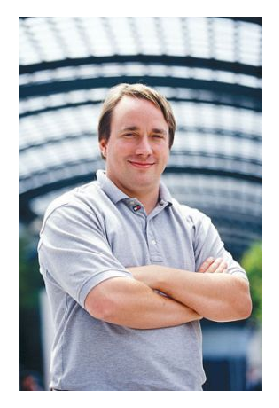
\includegraphics[width=4.0 cm]{./apa/linus_torvalds.eps}}
\end{psfrags}
{\small Fonte: Adaptado de \citeonline{machado}}
\end{center}
\label{torvalds}
\end{figure}

